% ! TEX root = ../mechanics.tex

%导弹飞行原理
\chapter{火箭导弹飞行原理}
\section{总空气动力}
\subsection{地面坐标系$Oxyz $}
发射点为原点$O$,弹道面与水平面
的交线为$Ox$轴,$Oy$轴在包含$Ox$的
铅锤面内,与$Ox$轴垂直,$Oz$轴按
右手螺旋法则确定.
\subsection{弹道坐标系$Ox_2y_2z_2$}
弹体质心为原点$O$,$Ox_2$轴与弹体质心
的速度矢量重合,$Oy_2$在包含$Ox_2$轴的
铅锤面内,并且与$Ox_2$垂直,$Oz_2$轴按
右手螺旋法则确定.
\subsection{速度坐标系$Ox_3y_3z_3$}
原点$O$在弹体的质心上,$Ox_3$轴与速度
矢量重合,$Oy_3$位于弹体纵向对称面内,
并与$Ox_3$垂直,$Oz_3$垂直于$Ox_3y_3$
平面,按右手螺旋法则确定方向.
\subsection{弹体坐标系$Ox_1y_1z_1$}
原点$O$取在弹体质心上,$Ox_1$与弹体
纵轴垂直,指向头部为正,$Oy_1$轴在弹体
纵向对称面内,垂直$Ox_1$轴,指向上方为正,
$Oz_1$垂直$Ox_1y_1$平面,按右手螺旋法则
确定方向.

两个坐标系都是动坐标系.

\begin{notice}
	\begin{enumerate}
		\item {\bfseries 攻角}\index{攻角}$\alpha$ \\
		      速度矢量$\mathbf{V}$在纵向对称平面
		      $Ox_1y_1$上的投影和$Ox_1$的夹角,若
		      $Ox_1$轴位于投影线的上方,则攻角$\alpha$
		      为正.
		\item {\bfseries 侧滑角}\index{侧滑角}$\beta$ \\
		      速度矢量$\mathbf{V}$在纵向对称平面$Ox_1y_1$
		      之间的夹角.若来流从右侧流向弹体则为正.(从
		      飞行方向观察)
        \item {\bfseries 俯仰角}\index{俯仰角}$\Xi$\\ 
          弹体纵轴$Ox_1$与水平面的夹角.
        \item {\bfseries 偏航角}\index{偏航角}$\Psi$\\ 
          弹体纵轴$Ox_1$在水平面内的投影与$Ox$的夹角.
        \item {\bfseries 滚转角}\index{滚转角}$\gamma$\\ 
          弹体坐标系$Oy_1$轴与包含弹体纵轴铅锤平面的夹角.
        \item {\bfseries 弹道倾角}\index{弹道倾角}$\theta$\\ 
          速度矢量$\mathbf{V}$与水平面的夹角.
        \item {\bfseries 弹道偏角}\index{弹道偏角}$\Psi_v$\\ 
          速度矢量$\mathbf{V}$在水平面内的投影与$Ox$的夹角.
        \item {\bfseries 速度倾斜角}\index{速度倾斜角}$\gamma_v$\\ 
          $Oy_3$与包含速度矢量$\mathbf{V}$的铅锤面的夹角.
	\end{enumerate}
	%tikz
	% ! TEX root = ./principle_of_flight.tex

\begin{center}

\tikzset{every picture/.style={line width=0.75pt}} %set default line width to 0.75pt        

\begin{tikzpicture}[x=0.75pt,y=0.75pt,yscale=-1,xscale=1]
%uncomment if require: \path (0,300); %set diagram left start at 0, and has height of 300

%Shape: Rectangle [id:dp1411189406840021] 
\draw  [fill={rgb, 255:red, 245; green, 166; blue, 35 }  ,fill opacity=1 ] (161.6,153.7) -- (392.24,99) -- (401.53,137.64) -- (170.89,192.34) -- cycle ;
%Straight Lines [id:da2938932926787814] 
\draw [color={rgb, 255:red, 74; green, 144; blue, 226 }  ,draw opacity=1 ]   (313.35,237.9) -- (265.85,51.2) ;
\draw [shift={(265.35,49.27)}, rotate = 75.72] [color={rgb, 255:red, 74; green, 144; blue, 226 }  ,draw opacity=1 ][line width=0.75]    (10.93,-3.29) .. controls (6.95,-1.4) and (3.31,-0.3) .. (0,0) .. controls (3.31,0.3) and (6.95,1.4) .. (10.93,3.29)   ;
%Straight Lines [id:da07973104503934425] 
\draw [color={rgb, 255:red, 126; green, 211; blue, 33 }  ,draw opacity=1 ]   (289.35,143.58) -- (361.8,85.27) ;
\draw [shift={(363.35,84.01)}, rotate = 141.17] [color={rgb, 255:red, 126; green, 211; blue, 33 }  ,draw opacity=1 ][line width=0.75]    (10.93,-3.29) .. controls (6.95,-1.4) and (3.31,-0.3) .. (0,0) .. controls (3.31,0.3) and (6.95,1.4) .. (10.93,3.29)   ;
%Straight Lines [id:da5051642498138564] 
\draw [color={rgb, 255:red, 126; green, 211; blue, 33 }  ,draw opacity=1 ]   (289.35,143.58) -- (225.65,68.66) ;
\draw [shift={(224.35,67.14)}, rotate = 49.63] [color={rgb, 255:red, 126; green, 211; blue, 33 }  ,draw opacity=1 ][line width=0.75]    (10.93,-3.29) .. controls (6.95,-1.4) and (3.31,-0.3) .. (0,0) .. controls (3.31,0.3) and (6.95,1.4) .. (10.93,3.29)   ;
%Straight Lines [id:da16788098204645885] 
\draw [color={rgb, 255:red, 126; green, 211; blue, 33 }  ,draw opacity=1 ]   (289.35,143.58) -- (374.69,200.06) ;
\draw [shift={(376.35,201.16)}, rotate = 213.5] [color={rgb, 255:red, 126; green, 211; blue, 33 }  ,draw opacity=1 ][line width=0.75]    (10.93,-3.29) .. controls (6.95,-1.4) and (3.31,-0.3) .. (0,0) .. controls (3.31,0.3) and (6.95,1.4) .. (10.93,3.29)   ;
%Straight Lines [id:da8889478781385203] 
\draw [color={rgb, 255:red, 74; green, 144; blue, 226 }  ,draw opacity=1 ]   (289.35,143.58) -- (256.08,229.08) ;
\draw [shift={(255.35,230.95)}, rotate = 291.26] [color={rgb, 255:red, 74; green, 144; blue, 226 }  ,draw opacity=1 ][line width=0.75]    (10.93,-3.29) .. controls (6.95,-1.4) and (3.31,-0.3) .. (0,0) .. controls (3.31,0.3) and (6.95,1.4) .. (10.93,3.29)   ;
%Straight Lines [id:da9590319678742609] 
\draw [color={rgb, 255:red, 74; green, 144; blue, 226 }  ,draw opacity=1 ]   (289.35,143.58) -- (373.85,102.55) ;
\draw [shift={(375.65,101.68)}, rotate = 154.1] [color={rgb, 255:red, 74; green, 144; blue, 226 }  ,draw opacity=1 ][line width=0.75]    (10.93,-3.29) .. controls (6.95,-1.4) and (3.31,-0.3) .. (0,0) .. controls (3.31,0.3) and (6.95,1.4) .. (10.93,3.29)   ;
%Straight Lines [id:da8595472323255129] 
\draw [color={rgb, 255:red, 208; green, 2; blue, 27 }  ,draw opacity=1 ]   (363.35,84.01) -- (375.65,101.68) ;
%Curve Lines [id:da30781488459018513] 
\draw    (332.5,122.63) .. controls (338.65,120.54) and (342.65,132.45) .. (334.65,133.44) ;
%Curve Lines [id:da3508432857182251] 
\draw    (326.35,113.8) .. controls (332.65,107.63) and (338.65,116.57) .. (332.5,122.63) ;
%Straight Lines [id:da500424813028004] 
\draw [color={rgb, 255:red, 80; green, 227; blue, 194 }  ,draw opacity=1 ]   (167.65,133.44) -- (207.88,154.36) ;
\draw [shift={(209.65,155.29)}, rotate = 207.48] [color={rgb, 255:red, 80; green, 227; blue, 194 }  ,draw opacity=1 ][line width=0.75]    (10.93,-3.29) .. controls (6.95,-1.4) and (3.31,-0.3) .. (0,0) .. controls (3.31,0.3) and (6.95,1.4) .. (10.93,3.29)   ;
%Shape: Triangle [id:dp056219082178769586] 
\draw  [fill={rgb, 255:red, 245; green, 166; blue, 35 }  ,fill opacity=1 ] (526.49,88.87) -- (401.53,137.64) -- (392.46,98.97) -- cycle ;
%Straight Lines [id:da07013554849919856] 
\draw [color={rgb, 255:red, 74; green, 144; blue, 226 }  ,draw opacity=1 ]   (87.15,191.44) -- (580.21,75.9) ;
\draw [shift={(582.15,75.44)}, rotate = 166.81] [color={rgb, 255:red, 74; green, 144; blue, 226 }  ,draw opacity=1 ][line width=0.75]    (10.93,-3.29) .. controls (6.95,-1.4) and (3.31,-0.3) .. (0,0) .. controls (3.31,0.3) and (6.95,1.4) .. (10.93,3.29)   ;

% Text Node
\draw (344.33,72.13) node [anchor=north west][inner sep=0.75pt]    {$\mathbf{V}$};
% Text Node
\draw (264.33,130.79) node [anchor=north west][inner sep=0.75pt]    {$O$};
% Text Node
\draw (560,79.32) node [anchor=north west][inner sep=0.75pt]    {$x_{1}$};
% Text Node
\draw (370,72.54) node [anchor=north west][inner sep=0.75pt]    {$x_{3}$};
% Text Node
\draw (274,47.04) node [anchor=north west][inner sep=0.75pt]    {$y_{1}$};
% Text Node
\draw (216.67,73.86) node [anchor=north west][inner sep=0.75pt]    {$y_{3}$};
% Text Node
\draw (247,198.59) node [anchor=north west][inner sep=0.75pt]    {$z_{1}$};
% Text Node
\draw (356,195.64) node [anchor=north west][inner sep=0.75pt]    {$z_{3}$};
% Text Node
\draw (345.33,112.59) node [anchor=north west][inner sep=0.75pt]    {$\alpha $};
% Text Node
\draw (345.67,91.71) node [anchor=north west][inner sep=0.75pt]    {$\beta $};
% Text Node
\draw (129,115.82) node [anchor=north west][inner sep=0.75pt]   [align=left] {纵向对称面};


\end{tikzpicture}
\end{center}

\end{notice}
\subsection{总空气动力}
{\bfseries 总空气动力}\index{总空气动力}可以
沿速度坐标系分解为升力$Y$,
阻力$X$,侧向力$Z$.
\begin{equation*}
	\begin{split}
		X&=C_x q S \\
		Y&=C_y q S \\
		Z&=C_z q S
	\end{split}
\end{equation*}
其中$q$是动压,$q=\frac{1}{2}\rho V^2$,
$S$是火箭的特征面积.$C_x$,$C_y$,$C_z$分别是
阻力系数,升力系数和侧向力系数.
\begin{note}
	空气动力的大小与来流的动压$q$和火箭的特征面积
	$S$成正比.
\end{note}
\begin{notice}
	\begin{enumerate}
		\item {\bfseries 升力}\index{升力} \\
		      全弹的升力可以看成是弹翼,弹身,尾翼(舵面)等
		      各部件产生的升力之和加上各部件之间相互干扰
		      的附加升力.弹翼是提供升力的主要部件,其余产
		      生的升力很小.

          升力系数基本上是马赫数,攻角,升降舵的舵面偏角的函数.
		      \begin{note}
			      升力系数大小与攻角有关,在一定范围内,攻角越大,升
			      力系数越大,超过之后,攻角再增大,升力系数急剧
			      减小,飞机失速.
		      \end{note}
        \item {\bfseries 侧向力}\index{侧向力}\\ 
          侧向力系数基本上取决于马赫数,侧滑角,
          方向舵舵面偏转角.
		\item {\bfseries 阻力}\index{阻力} \\
		      作用在火箭导弹上的总空气动力在速度方向上的分量
		      就是阻力,它总是与速度方向相反,起到阻碍火箭导弹
		      运动的作用.
		      \begin{note}
			      阻力受空气的粘性影响最为显著.
		      \end{note}
		      导弹的空气阻力通常被分为两部分.
		      \begin{enumerate}
			      \item {\bfseries 零升阻力}\\
			            升力为零时的阻力.分为摩擦阻力和压差阻力.
			      \item {\bfseries 诱导阻力}\\
			            由升力或侧向力诱导出来的阻力(即与升力或者
			            侧向力大小有关).
		      \end{enumerate}
          诱导阻力是伴随升力而产生的,没有升力也就没有诱导阻力.
	\end{enumerate}
\end{notice}

\section{总空气力矩}
将总空气力矩沿弹体坐标系分解为三个分量,分别为
滚转力矩$M_x$,偏航力矩$M_y$,俯仰力矩$M_z$,气动
力矩的表达式为
\begin{equation*}
  \begin{split}
    M_x&=m_x q S L\\ 
    M_y&=m_y q SL \\ 
    M_z&=m_z q SL 
  \end{split}
\end{equation*}
其中,$m_x $,$m_y $,$m_z $
分别是滚转力矩,偏航力矩,俯仰力矩,统称为
气动力矩系数.$L$是特征长度,通常选弹身长
度为特征长度.
\begin{notice}
\begin{enumerate}
  \item {\bfseries 俯仰力矩}\index{俯仰力矩}\\ 
    俯仰力矩又称纵向力矩,控制导弹绕横轴$Oz_1$作
    抬头或低头的转动.在气动布局和外形系数给定的情况下,
    俯仰力矩是飞行马赫数,飞行攻角,飞行高度,操纵面偏转角,
    导弹绕$Oz_1$轴转动的角速度,攻角的变化率,操纵面的偏转角速度
    的函数.
  \item {\bfseries 偏航力矩}\index{偏航力矩}\\ 
    偏航力矩使导弹绕$Oy_1$轴转动
  \item {\bfseries 滚转力矩}\index{滚转力矩}\\ 
    滚转力矩使导弹绕$Ox_1$轴转动,是由迎面气流
    不对称地流过导弹造成的.

    滚转力矩的大小取决于导弹的外形和尺寸,飞行速度和高度,
    攻角,侧滑角,舵面及副翼的偏转角速度,以及制造误差等
  \item {\bfseries 铰链力矩}\index{铰链力矩}\\ 
    当操纵面偏转一个角度时,在操纵面上产生空气动力.
    它除了产生使火箭绕质心转动的力矩外,还产生相对于
    操纵面铰链轴的力矩,称为铰链力矩.
\end{enumerate}
\end{notice}
\subsection{压力中心和焦点}
总空气动力的作用线和导弹纵轴的交点称为
全弹的{\bfseries 压力中心}\index{压力中心}.
\begin{note}
在攻角不太大的情况下,可以近似地将全弹升力
作用线和纵轴的交点看作压力中心.
\end{note}
{\bfseries 焦点}\index{焦点}:由攻角$\alpha$
引起的那部分升力$Y^a_\alpha$的作用点称为焦点.
该点位于纵向
对称面内,升力对于通该点且平行于$Oz_1$轴的力矩
与攻角无关.
\begin{note}
压心和焦点一般不重合,仅在$\delta_z=0$,且
火箭导弹相对于$x_1Oz_1$平面完全对称时才重合.
\end{note}
\section{马格努斯效应}
如下图,
\begin{figure}[!ht]
  \centering
  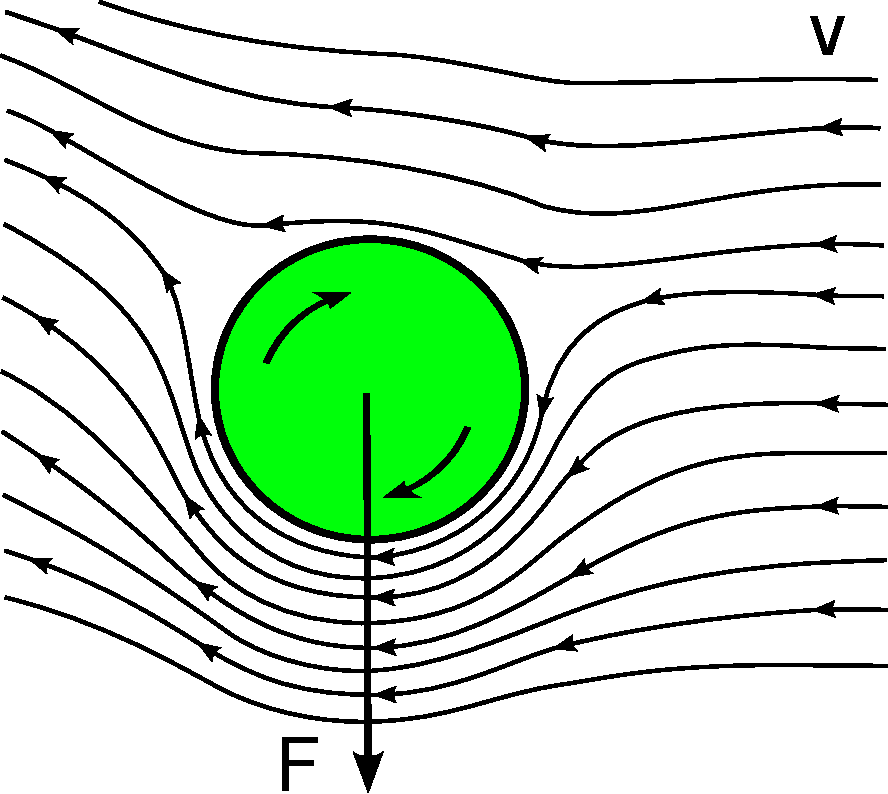
\includegraphics[width=5cm]{./Introduction_to_rocket_missile_tec/Magnus_effect.pdf}
\end{figure}
弹体绕自身对称轴旋转,使得两侧的的压强大小不一致,产生一个横向力$F$.

\section{火箭运动方程}
火箭在瞬时$t$的质量$M$和原质量$M_0$的关系时
\[
  M=M_0-\int_0^t \dot{m}\mathrm{d}t
\]
其中$\dot{m}$是质量变化率,为负值.
不考虑重力和气动力的情况下,火箭的速度称为理想速度,
是仅在发动机推力作用下火箭的速度.
于是
\[
  \mathrm{d}v=-u_e \frac{\mathrm{d}M }{M }
\]
也就是
\[
  v=-u_e \ln \frac{M}{M_0}
\]
记$\frac{M}{M_0}$为$\mu$,故火箭的理想末速度是
\begin{empheq}[box=\bluebox]{equation*}
  v_k=-u_e \ln \mu_k
\end{empheq}
\begin{note}
$\mu_k$是火箭的结构系数,是表示火箭结构设计优劣的一个
重要参数,用来衡量火箭的结构性能,$\mu_k$越小,火箭的速
度越大.
\end{note}
\begin{notice}
提高火箭的理想速度的两个方法:
\begin{enumerate}
  \item 提高燃气流的喷速$u_e$
  \item 降低火箭的结构系数$\mu_k$
\end{enumerate}
\end{notice}
\begin{example}
  现有一三级火箭,燃气的喷速均为$2200$m/s,结构
  系数均为$0.2$,求火箭的理想末速度.
  \[
    v=-3u_e \ln \mu_k=-3\times 2200\times \ln 0.2=10600\text{m/s}
  \]
\end{example}


